\documentclass{article}
\usepackage[letterpaper,top=2cm,bottom=2cm,left=3cm,right=3cm,marginparwidth=1.75cm]{geometry}
\usepackage{amsmath}
\usepackage{graphicx}
\usepackage[backend=biber, style=ieee]{biblatex}
\usepackage[vietnamese]{babel}

\newcommand{\mylogo}{
\includegraphics[width=5cm]{logo.png}}

\begin{document}
\begin{titlepage}
\begin{center}
    \fontsize{18}{22}\selectfont
    TRƯỜNG ĐẠI HỌC CÔNG NGHỆ\\
    ĐẠI HỌC QUỐC GIA HÀ NỘI
\end{center}
\vspace{1cm}
\centering
\mylogo 
\vspace{2cm}

\Huge{Mô phỏng hiện tượng bày đàn}\\[1ex]
\vspace{3cm}
\begin{flushleft} 
    \fontsize{17}{12}\
    \textbf{Giảng viên:} Nguyễn Hồng Thịnh \\
    \textbf{Nhóm thực hiện:} Nhóm 2 \\
    \hspace{4em} 21021600 - Lương Quốc Khánh \\
    \hspace{4em} 21020698 - Nguyễn Đức Minh \\
    \hspace{4em} 21020688 - Đỗ Huy \\
    \hspace{4em} 21021587 - Phạm Minh Hiếu \\
\end{flushleft}
\end{titlepage}
\section{Giới thiệu}

Lập trình Python sử dụng thư viện pygame mô phỏng hiện tượng bầy đàn. Thông qua chương trình ta có thể tìm hiểu, điều chỉnh về những tác động làm ảnh hưởng đến tập cá thể.
Trong ứng dụng này, chúng tôi có các cá thể là những hình ô vuông màu xanh được mô phỏng bên trái màn hình, bên phải là màn hình điều chỉnh độ lớn của các tác động cũng như tăng giảm số lượng cá thể biểu diễn và tốc độ di chuyển của chúng.

\begin{figure}[htbp]
  \centering
  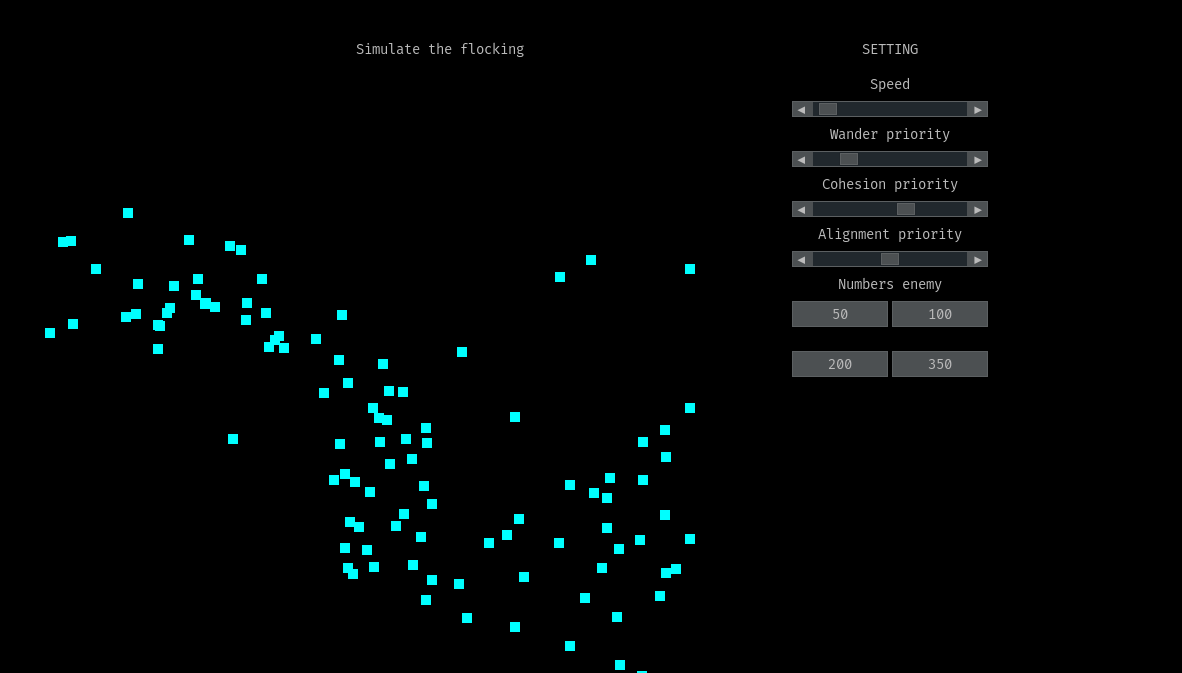
\includegraphics[width=0.5\linewidth]{demo.png} 
  \caption{Màn hình làm việc.}
\end{figure}

Các tác động xử lý:
\begin{enumerate}
\item Sự ngẫu nhiên: cá thể di chuyển ngẫu nhiên, không theo quy luật nào.
\item Sự kết hợp: cá thể di chuyển về hướng của bầy đàn.
\item Sự giãn cách: cá thể di chuyển tránh va chạm với các cá thể khác.
\end{enumerate}
Sự kết hợp các tác động giúp tạo nên chương trình của chúng tôi. Chúng tôi mong rằng nó sẽ hữu ích và khơi gợi sự hứng thú của bạn về chủ đề này.

\section{Các tác động.}

\subsection{Tác động ngẫu nhiên.}
Sự ngẫu nhiên có thể xảy ra bất cứ lúc nào và không có dự đoán trước theo một quy luật nào đó. Bằng cách tạo một hướng đi mới ngẫu nhiên kết hợp với hướng đi ban đầu rồi chuẩn hóa chúng tôi biểu diễn được được di chuyển ngẫu nhiên của cá thể.\\

\begin{figure}[htbp]
  \centering
  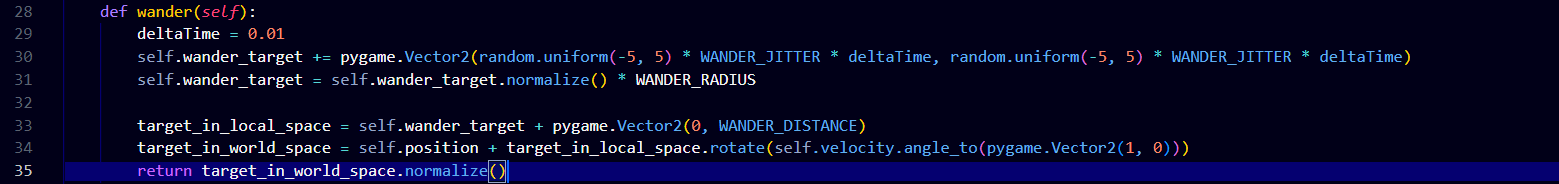
\includegraphics[width=0.5\linewidth]{wander.png} 
  \caption{Xử lý dữ liệu trên python.}
\end{figure}
\vspace{3cm}
\subsection{Tác động kết hợp.}
Bằng cách tổng hợp hướng di chuyển của cá thể đồng loại xung quanh và nằm trong hướng quan sát rồi chia cho số lượng cá thể rồi chuẩn hóa nó, chúng tôi tính được vector vận tốc cần di chuyển.\\
\begin{figure}[htbp]
  \centering
  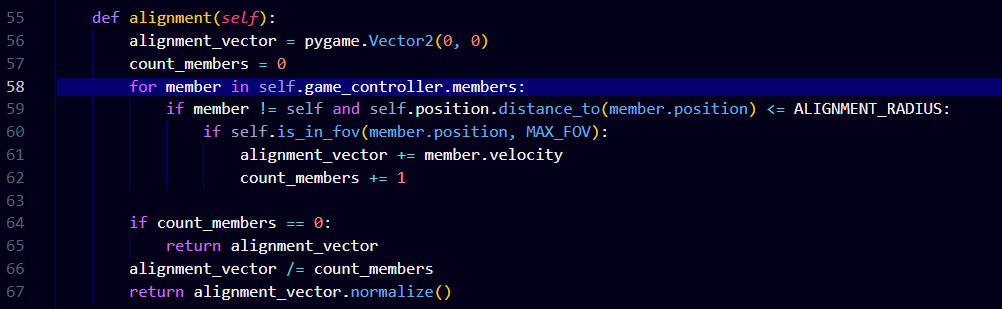
\includegraphics[width=0.5\linewidth]{alignment.png} 
  \caption{Xử lý dữ liệu trên python.}
\end{figure}

Trong đó:
\begin{itemize}
\item alignmentVector là vận tốc mới cần căn chỉnh.
\item ALIGNMENT RADIUS là bán kính ảnh hưởng.
\item countMembers là số lượng cá thể thỏa mãn.
\item self.gameController.members là tập các cá thể.
\end{itemize}


\subsection{Tác động giãn cách}
Bằng cách tổng hợp vị trí của các cá thể nằm trong phạm vi xét sau đó lấy trung bình vị trí tổng hợp trừ đi vị trí hiện tại ta được vector hướng. Tiếp tục chuẩn hóa ta được kết quả cần tính.\\
\begin{figure}[htbp]
  \centering
  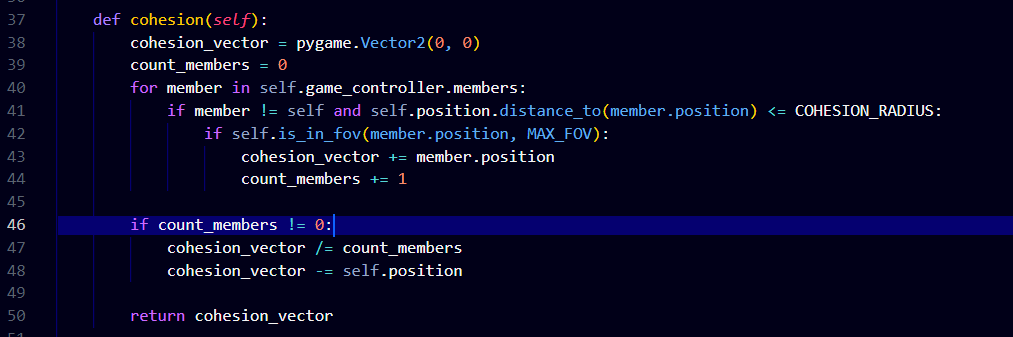
\includegraphics[width=0.5\linewidth]{cohesion.png} 
  \caption{Xử lý dữ liệu trên python.}
\end{figure}

Trong đó:
\begin{itemize}
\item cohesionVector là vận tốc mới cần căn chỉnh.
\item COHESION RADIUS là bán kính ảnh hưởng.
\item countMembers là số lượng cá thể thỏa mãn.
\item self.gameController.members là tập các cá thể.
\end{itemize}


\section{Xử lý UI}
Thông qua thư viện pygameGui trong python chúng tôi thiết lập những thanh kéo (slider) để điều chỉnh chỉ số ảnh hưởng của các tác động với cá thể, nút bấm (button) để điều chỉnh số lượng cá thể trong mô phỏng.
\begin{figure}[htbp]
  \centering
  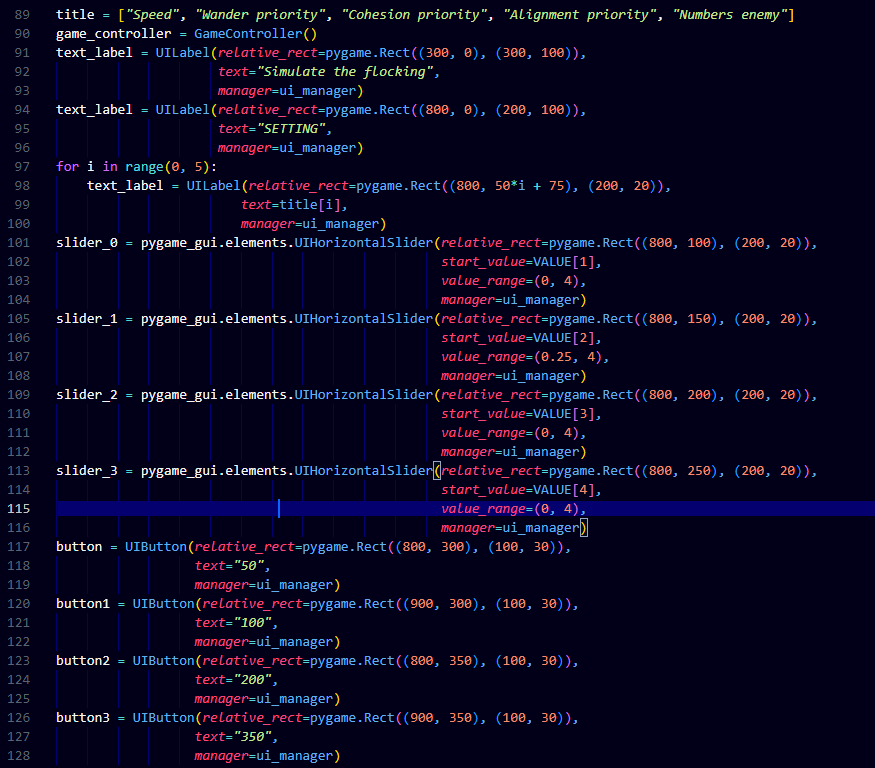
\includegraphics[width=0.5\linewidth]{UI1.png} 
  \caption{Cài đặt các nút bấm và thanh kéo.}
\end{figure}
\begin{figure}[htbp]
  \centering
  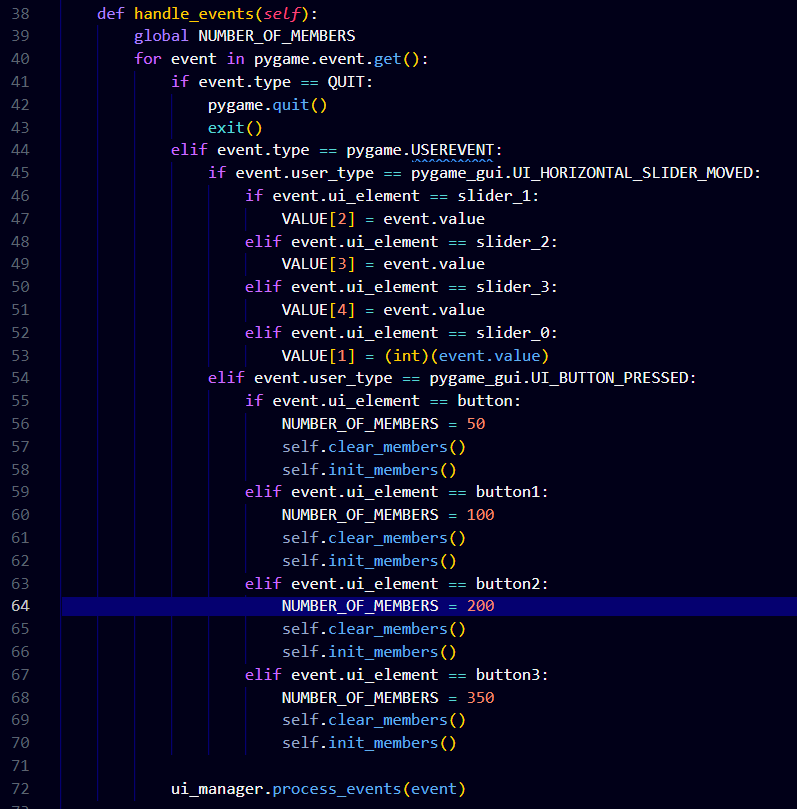
\includegraphics[width=0.5\linewidth]{UI2.png} 
  \caption{Xử lý logic.}
\end{figure}

\section{Kết luận}

Trong quá trình thực hiện mô phỏng hiện tượng bày đàn sử dụng thư viện pygame, chúng tôi đã thành công trong việc tạo ra một chương trình linh hoạt và sinh động, giúp hiểu rõ hơn về cách các cá thể trong bầy đàn tương tác với nhau. Bằng cách kết hợp các tác động như ngẫu nhiên, kết hợp và giãn cách, chúng tôi đã tạo ra một mô phỏng sống động về hành vi của các cá thể trong một bầy đàn.

Hình ảnh minh họa trong màn hình làm việc (Hình 1) đã thực sự thể hiện sự linh hoạt và tính chân thực của mô phỏng của chúng tôi. Việc điều chỉnh các tham số như bán kính ảnh hưởng và số lượng cá thể đã giúp chúng tôi quan sát được sự biến đổi đáng kể trong hành vi của bầy đàn.

Các tác động như ngẫu nhiên, kết hợp và giãn cách đã được hiện thực một cách chặt chẽ và thực tế, giúp chúng tôi đạt được mục tiêu mô phỏng một cách chân thực và hấp dẫn. Hy vọng rằng chương trình mô phỏng của chúng tôi sẽ là nguồn cảm hứng cho các nghiên cứu về hiện tượng bày đàn và sẽ thúc đẩy sự hiểu biết về tương tác giữa các cá thể trong tự nhiên.
\end{document}